\documentclass[12pt,a4paper]{article}

% --- Encoding & fonts (XeLaTeX) ---
\usepackage{fontspec}
\setmainfont{Times New Roman}
\setmonofont{Courier New}

% --- Language ---
\usepackage{polyglossia}
\setdefaultlanguage{english}

% --- Math ---
\usepackage{amsmath,amssymb,amsthm}
\usepackage{unicode-math}
\usepackage{booktabs}
\usepackage{array}
\usepackage{tabularx}
\usepackage{graphicx}
\usepackage{caption}
\captionsetup{labelfont=bf, textfont=it}
\usepackage{longtable}

% --- Page layout ---
\usepackage[a4paper, margin=2.5cm, bottom=3cm]{geometry}
\usepackage{setspace}
\onehalfspacing
\raggedbottom

% --- Typography ---
\usepackage{microtype}
\usepackage[stable]{footmisc}
\frenchspacing

% --- Running header / footer ---
\usepackage{fancyhdr}
\pagestyle{fancy}
\fancyhf{}
\fancyhead[L]{\small A Structural Microsimulation of a Neighborhood Grocery Store}
\fancyhead[R]{\small Chinh Mai}
\fancyfoot[C]{\thepage}
\renewcommand{\headrulewidth}{0.4pt}

% --- Hyperlinks ---
\usepackage[colorlinks=true,linkcolor=blue,citecolor=blue,urlcolor=blue]{hyperref}

% --- Lists ---
\usepackage{enumitem}
\setlist{leftmargin=*, topsep=6pt, itemsep=4pt, parsep=0pt}

% --- Diagrams ---
\usepackage{tikz}
\usetikzlibrary{positioning, arrows.meta, shapes.geometric, fit, backgrounds}

\title{\textbf{Two Layers of an Economy:\\
Decisions, Scripts, and the Anatomy of a Simulated Grocery Store}}
\author{Chinh Mai}
\date{July 2026}

\begin{document}

\maketitle

\begin{abstract}
This paper tells the story of a simulated small grocery store from the
ground up: not by walking through the software that builds it, but by
walking through the economic decisions that give it its shape. Every
number this construction produces --- a receipt, an invoice, a monthly
ledger, a tax filing --- is the residue of somebody choosing something. A
customer chooses between two cartons of milk. An owner chooses where to
open a store before a single customer has walked through the door. The
same owner chooses, later, whether to hire, and whether to expand, under
capital he does not have room to lose. This paper follows each of those
choices from the plain human intuition behind it to the precise
mathematical object that intuition becomes, and does the same for the one
thing in this world that is never a choice at all: the weather, the
calendar, and the macroeconomic shocks that are scripted in advance and
never listen to anything the simulated people do. That distinction ---
between what is chosen and what is merely scripted --- is not a modeling
convenience. It is what allows a later reader to ask what would have
happened without the storm, or without the competitor, and receive an
answer that is exactly true rather than merely estimated. The result is
intended as a companion for anyone who wants to understand this
simulated economy in its own right, whether or not they ever open the
software that runs it; readers who want the precise specification of
every mechanism, at a level suitable for reimplementation, should consult
\texttt{documents/PHASE1\_DETAILS.md} through \texttt{PHASE5\_DETAILS.md}
in the project repository, which this paper deliberately does not
duplicate.
\end{abstract}

\clearpage

\section{Two Layers of an Economy}
\label{sec:intro}

Suppose you hand a new analyst a spreadsheet and tell her it is real. She
has no way to check whether her conclusions are correct, only whether
they sound reasonable, because nobody --- not her, not you, not the
business itself --- actually knows the true mechanism that produced the
numbers. Now suppose instead you hand her a spreadsheet you generated
yourself, by drawing every column from a convenient distribution. She can
check her work against your generating code, but there is nothing
underneath the numbers worth discovering: no owner who misread a signal,
no competitor who actually mattered less than everyone assumed, no honest
mess in the paperwork to clean up before the real question can even be
asked. Teaching data analysis with either kind of data teaches half the
job.

This paper is about a third option: build the business first, as a world
with people, budgets, and a street, and only afterward let the paperwork
fall out of what that world actually did. Do that carefully enough, and
you get something rare --- a dataset messy enough to feel real, and yet
one where every number still has a traceable cause, so a conclusion can
be checked not just for plausibility but for truth.

\subsection{An economy is a collection of decisions}

Every column in a business's ledger is the fossil record of somebody
choosing something: a customer choosing a shelf, an owner choosing a
price, a bank choosing a loan. \emph{If data is going to teach real
analysis, it has to model the choosing, not the ledger.} This construction
takes that literally. It contains no column that was not produced by a
decision --- a customer's, an owner's, or in one case a whole population's
slow drift in and out of a neighborhood --- and every decision is built
the same way, in three steps that recur throughout this paper: first the
plain economic intuition behind the choice, in language you would use to
explain it to a friend; then the nature of the choice itself, meaning what
kind of decision problem it structurally is, a discrete pick among a
handful of options, a one-shot allocation of scarce capital, a threshold
crossed or not; and finally the precise stochastic process that
intuition becomes once it is written in the language of mathematics.

Meet Henrik Fjeld. He is not a real person --- his name, his age, and the
street he lives on are invented for each run of this simulation, chosen
fresh from a small cast of possibilities every time someone generates a
new store. But everything that happens to his shop is not invented at
all: it is the exact, computed consequence of decisions made by
simulated people responding to a simulated world, the same way a real
ledger is the consequence of decisions made by real people responding to
a real one. Consider one such decision, small enough to hold in your
head. A customer walks into Henrik's shop wanting a carton of milk. Two
sit on the shelf: a familiar national brand at \texttt{\euro{}1.89}, and
the store's own cheaper label at \texttt{\euro{}1.49}. She does not
compute anything --- she just knows, the way you know at the supermarket,
that today the cheaper one will do just fine, but last week, buying for a
dinner guest, only the brand name felt right. That is the entire
economic content of the decision: a comparison between an option's price
and how much she happens to want the thing the price difference buys.
Section~\ref{sec:micro} turns that comparison into the single equation
that governs every purchase in this economy, and Table~\ref{tab:milk}
there shows the same customer, the same two cartons, and the one thing
that actually changed between two different Tuesdays.

\subsection{What is scripted and what is chosen must never be confused}

Multiply Henrik's customer's decision by three hundred households, three
years, and every shelf in the store, and you get something that looks,
from the outside, exactly like a real small business: a ledger with good
months and bad ones, a competitor who opens down the street and costs
the owner something --- though maybe not what he thinks it costs him ---
and a set of records honest enough to contain the ordinary mistakes a
real bookkeeper makes. From the inside, though, every one of those
numbers still traces back to a decision like Henrik's customer and her
milk: a person, a comparison, a choice.

This is also where the model draws a line that is never allowed to
blur. A storm, a tax change, a competitor's arrival are written into the
world in advance, on a specific date, independent of anything anyone in
the simulation does. A customer's purchase, an owner's price, an owner's
decision to hire are never written down anywhere at all --- they emerge,
fresh, from the decision-maker's own situation each time the world is
run. \emph{What is scripted and what is chosen are never allowed to be
confused.} Keeping that line sharp is what lets a later section ask
``what would have happened without the storm?'' and get back an answer
that is exactly true, rather than merely estimated, because nothing
about the storm could possibly have been caused by anything the shop's
own people did.

Two layers follow from this one distinction, and this paper is organized
around exactly the two of them. Section~\ref{sec:micro}, \textbf{the
micro layer}, walks through every kind of decision this simulated world
contains: what a customer wants, what an owner believes before he has a
single sale to go on, when an owner dares to expand, and who stays a
customer and who drifts away. Nothing in this layer is written down in
advance; everything in it is computed fresh, each time the world is run,
from the situation the decision-maker actually faces.
Section~\ref{sec:macro}, \textbf{the macro layer}, covers everything
that \emph{is} written down in advance: the calendar, the weather,
macroeconomic shocks, and the tax code the whole economy operates
under. Section~\ref{sec:counterfactual} explains why keeping these two
layers from ever talking to each other in the wrong direction is what
makes this world useful for more than description --- it is what lets
a later reader ask a genuine causal question and trust the answer.
Section~\ref{sec:recording} covers a third thing that is neither a
decision nor a script: the paperwork itself, which is allowed to be
wrong in small, realistic ways even though the world underneath it never
is. Section~\ref{sec:literature} places this construction against the
other ways synthetic and case-study business data are made today, and
Section~\ref{sec:discussion} steps back to ask what the whole
architecture buys, and for whom.

The goal of everything that follows is not to prove a theorem. It is to
leave a reader able to open Henrik Fjeld's ledger, or the ledger of the
next store this same machinery generates under a different roll of the
dice, and already know, before running a single regression, what kind
of story could possibly be hiding inside it.

\section{Related Approaches and the Case for Structural Synthesis}
\label{sec:literature}

Synthetic business data is not a new idea, and it is worth being precise
about where this construction sits relative to approaches already in
routine use. Four traditions dominate the current landscape, each built
to optimize for something other than what this project optimizes for.

\subsection{Rule-based generators}

The simplest and most widely used tools, such as Faker and Mockaroo, fill
a schema with plausible-looking field values: names, addresses, dates,
amounts drawn from simple parametric distributions attached
independently to each column. These tools are fast and entirely adequate
for their actual purpose, populating a database or testing a software
pipeline against realistically shaped inputs. They are not built to
support analysis practice, because each column is generated independently
of every other: there is no mechanism linking a customer's income to
their basket size, no mechanism linking weather to foot traffic, and no
sense in which the resulting numbers were caused by anything. A student
who regresses one generated column on another is not discovering a
relationship, because none was ever built in.

\subsection{Statistical and generative model synthesizers}

A more sophisticated family of tools learns to imitate the statistical
shape of a real dataset rather than sampling columns independently.
Conditional generative adversarial networks such as CTGAN, variational
autoencoders, and copula-based tools bundled in synthesis libraries such
as the Synthetic Data Vault (\hyperlink{ref:patki2016}{Patki, Wedge, and
Veeramachaneni, 2016}; \hyperlink{ref:xu2019}{Xu, Skoularidou,
Cuesta-Infante, and Veeramachaneni, 2019}) are trained on a real seed
dataset and learn to reproduce its marginal distributions and pairwise
correlations closely enough to substitute for it in downstream use,
often motivated by a differential privacy guarantee
(\hyperlink{ref:dwork2006}{Dwork, 2006}). This is a genuine and valuable
technology for privacy-preserving data sharing, and a poor fit for
teaching data analysis, for three reasons. It requires an existing real
dataset to imitate, so it cannot manufacture a genuinely new case. The
generator itself is a black box, reproducing a distribution's shape
without asserting any mechanism that produced it, so there is no known
ground truth against which a causal claim can be graded. And a
distribution-matching model has no way to answer a counterfactual
question at all, because it was never given a reason for any number,
only a shape to reproduce; asking such a model what revenue would have
been without a tax change is not merely hard, it is category confusion.

\subsection{The business case method}

Business schools have long taught with hand-authored cases: a narrative
description of a company's situation accompanied by a set of exhibits,
built by a case writer around a specific pedagogical point. This
tradition, associated most closely with Harvard Business School's case
method, remains the gold standard for teaching judgment under ambiguity,
and the persona-and-letter device this project's own case briefs use
(Section~\ref{sec:micro}) borrows directly from it. Its limitation is not
narrative quality but process: each case is bespoke, manually tuned by
its author to make the numbers come out right, produced once, and reused
unchanged for years. There is no underlying generative process to
interrogate, no way to produce a counterfactual twin of the same company
under a different tax regime, and no way to grade a causal claim against
a documented mechanism, because the case writer's spreadsheet is the only
ground truth that exists, and it was authored to support a conclusion
rather than to allow one to be discovered.

\subsection{Structural microsimulation}

The methodological tradition closest to this project's own is structural
microsimulation, founded by \hyperlink{ref:orcutt1957}{Orcutt's (1957)}
proposal to model an economy as a population of individual units
following explicit behavioral rules rather than aggregate equations, and
carried forward today in tax and benefit microsimulation models such as
EUROMOD and in agent-based market and transport simulations across
applied economics. These models share this project's central
commitment: agents obey genuine, documented behavioral rules, so a
policy change can be replayed through an unchanged population and the
difference is a true causal effect. Where they typically diverge is in
what they are built to produce --- an aggregated statistic destined for
a policy briefing rather than a transaction-level business record --- and
because their audience is professional economists rather than students
learning to reconcile data, they rarely simulate imperfect paperwork,
since a policy model has no reason to misfile an invoice.

\subsection{What this construction combines}

No single tradition above combines all four of the properties this
project requires at once: a fully documented structural generating
process rather than a black box; transaction-level business artifacts
carrying deliberately realistic, separately documented paperwork
imperfections; exact counterfactual replay at the level of individual
decisions, made possible only by the keyed-randomness discipline of
Section~\ref{sec:counterfactual}; and a built-in scorecard for the analysis
itself, three profit figures (Section~\ref{sec:micro}) that turn the
abstract idea of analytical value into a specific, computed number ---
the gap between what an owner believed, what he actually earned, and
what a perfectly informed operator could have earned. None of the four
traditions above stage a protagonist who is wrong in a way that can be
measured.

\subsection{Value for teaching scientific reasoning, not only data analysis}

The deeper claim behind this construction is that its principal teaching
value is not technical fluency with a particular software tool but a
disciplined scientific habit of mind, and that a dataset with a fully
known generating process is uniquely suited to teaching that habit
because it can tell a learner, definitively, when they are right. An
analyst working this data is repeatedly placed in a position where a
plausible-looking pattern is a trap rather than a finding: a flat
category (Section~\ref{sec:macro}) whose apparent seasonality is a
budget-mediation effect rather than a genuine preference, a markdown
campaign (Section~\ref{sec:micro}) whose naive before-and-after
comparison is contaminated by the very selection rule that triggered it,
an energy crisis (Section~\ref{sec:macro}) whose use as a price
instrument is subtly invalid because it also moves household budgets.
Each trap has a documented, correct resolution, which means an
instructor can teach the general scientific skill of interrogating one's
own inference by handing a learner a specific claim, a specific method
for checking it, and a specific ground truth that reveals whether the
checking actually worked.

\section{The Micro Layer: Economic Decisions from the Ground Up}
\label{sec:micro}

Everything in this section shares one property: nothing in it is written
down anywhere in advance. A customer's purchase, an owner's price, an
owner's decision to hire, a household's decision to move away --- these
are computed fresh, each time the world is run, from the situation the
decision-maker actually faces at that moment. This section walks through
five such decisions, in the order a real small business actually
encounters them: what a customer wants at the shelf; what an owner
believes and decides before a single customer exists; how that same
owner adjusts, day to day, once real customers do exist; when the owner
dares to risk capital on growing the business; and, last, a kind of
motion that is not really a decision at all but a population's slow
drift, which this section includes anyway because it is exactly as
emergent, and exactly as stochastic, as everything else here.

\subsection{The customer's purchase decision}
\label{sec:micro-customer}

Consider Henrik Fjeld's customer again. She does not walk in with a
spreadsheet. She walks in wanting milk, glances at two cartons, and buys
one, and if you asked her why, she would give you a sentence, not an
equation: \emph{the cheap one is fine today}, or \emph{I want the good
one, since I have a guest}. Every real purchase decision this store will
ever record is, underneath, one of these small sentences, repeated by
three hundred different people with three hundred different budgets and
tastes, at every shelf in the store, every day for three years.

Structurally, this is what economists call a discrete choice: a customer
facing a small, enumerable set of alternatives --- the products on one
shelf, plus the option of buying nothing here at all --- picks exactly
one. It is not a continuous decision like choosing how much to spend;
it is a pick. What makes the pick interesting is that it depends on
three separate things at once: how much the customer currently needs the
category at all, how well each product on the shelf actually matches her
taste, and how much each one costs relative to what she is willing to
pay. A rich model of this decision has to hold all three considerations
in the same comparison, rather than resolving need, taste, and price one
after another as though they did not interact.

Put the sentence into the language of mathematics, and it becomes a
single expression. Each product $s$ offers a customer $i$ a utility

\[
U_{is} = \theta_{ic} + a_s + \gamma\left(1 - \left|b_i -
\text{BrandLevel}_s\right|\right) - \beta_i\,\text{Price}_s ,
\]

where $\theta_{ic}$ is the customer's current need for the category. The
term $b_i$ is her brand affinity, $\text{BrandLevel}_s$ is the product's
own position on that same spectrum, and the middle term rewards a good
match between the two, with $\gamma$ setting how much that match matters.
$\beta_i$ is her own price sensitivity, and $a_s \sim \text{Normal}(0,
0.8)$ is an unmodeled per-product appeal intercept, standing in for the thousand
unmodeled reasons one product outsells its shelf neighbor, such as
packaging or familiarity. Alongside every stocked product sits an
outside option, representing the choice to buy nothing here or to buy
elsewhere, and the actual choice is drawn as

\[
\text{choice} \sim \text{Categorical}\big(\text{softmax}(U_{is_1}, \ldots,
U_{is_K}, U_0)\big) .
\]

The softmax form is not a convenient approximation; it is the exact
consequence of a well-known result in discrete choice theory. If each
product's utility is disturbed by an independent, identically
distributed Gumbel shock and the customer simply picks the option with
the highest noisy utility, the resulting choice probabilities are
exactly the softmax of the mean utilities --- McFadden's random utility
result (\hyperlink{ref:mcfadden1974}{McFadden, 1974}). The smooth
formula above and the human story of a shopper with genuine but noisy
tastes are the same model described two ways, and it happens to be
exactly the model a real discrete-choice analyst would fit to purchase
histories, so grading a later analytical exercise against the true
parameters is a fair comparison of like against like.

Table~\ref{tab:milk} makes the same point in a different medium. It
scores Henrik's customer's utility for both cartons on two different
occasions --- an ordinary Tuesday, and the evening she is shopping for a
dinner guest --- decomposed into exactly the terms the equation named.

\begin{table}[htbp]
\centering
\begin{tabular}{lcc}
\toprule
& Ordinary Tuesday & Dinner guest \\
\midrule
Brand match, $\gamma(1-|b_i - \text{BrandLevel}_{\text{brand}}|)$ & $0.60$ & $0.60$ \\
Brand match, $\gamma(1-|b_i - \text{BrandLevel}_{\text{store}}|)$ & $0.50$ & $0.50$ \\
Price term, $\beta_i \cdot$ price difference & $-0.40$ & $-0.40$ \\
$a_s$ (that day's unmodeled pull) & $-0.05$ & $+0.35$ \\
\midrule
$U_{\text{brand}} - U_{\text{store}}$ & $-0.35$ & $+0.45$ \\
Chosen carton & store brand & national brand \\
\bottomrule
\end{tabular}
\caption{One customer, one choice, two occasions. Quality and price
enter identically both times; only the unmodeled pull term changes ---
and it alone flips which carton wins.}
\label{tab:milk}
\end{table}

Nothing in the table is new information; it is the same equation, the
same customer, and the same two cartons of milk, rearranged so that the
one thing that actually changed --- not her taste, not the prices, only
the part of that day even she could not fully explain --- is the one
thing the eye lands on first.

This single structure produces, without any additional machinery, four
properties a realistic market must have. Demand slopes downward, because
raising a product's price lowers its utility and therefore its choice
probability, at a rate set by each customer's own price sensitivity.
Substitution follows a sensible pattern, because a price increase on one
product pushes probability mass onto its nearest neighbors in brand
level, not onto arbitrary alternatives. Budget discipline emerges
naturally, because a customer works through a shopping list item by item
until the budget binds. And hidden demand is recorded automatically:
when a customer's first choice is out of stock, the original choice is
logged as a latent truth before she re-evaluates the softmax over what
remains, giving an honest ledger of demand that never appears in the
sales data at all.

That last property deserves its own sentence, because it is what turns
this decision from a single equation into a genuine daily market. A
visiting customer's need for a category is driven by a pantry: a latent
stock that drains at a steady rate and refills only when she actually
buys more, $P_{ic,t+1} \overset{\leftarrow}{=} \max(0,\ P_{ict} -
r_{ict}) + \text{units purchased}$, with the drain rate itself scaled by
the season's demand modifier rather than added to her desire directly,
so a hot week does not make a household want ice cream in the abstract,
it makes the household eat the ice cream in the freezer faster. Her need
for the category, $\theta_{ict} = \alpha\,\max(0,\ P^{\text{tgt}}_{ic} -
P_{ict})/P^{\text{tgt}}_{ic}$, is exactly the shortfall against a target
of ten days' comfortable cover, and it is this shortfall, not a fresh
random draw, that feeds $\theta_{ic}$ in the utility equation above. When
her chosen product is unavailable, three things happen in order: the
original intent is logged as a latent truth under the cause
\texttt{stockout}; the same softmax is re-evaluated with that product
removed, so probability mass flows to its nearest neighbors exactly as
the substitution story above predicts; and if the re-evaluated choice
still lands on the outside option, the store has lost a sale it will
never observe in its own data. Four distinct causes of invisible demand
accumulate this way over a year --- an arrival outside opening hours, a
stockout, an exhausted weekly budget partway through the list, and the
outside option simply winning on price --- and together they are the
honest, mechanistic version of the familiar claim that sales data are
demand data, censored in several distinct ways, each with its own
recorded cause.

\subsection{The owner's opening decision}
\label{sec:micro-opening}

Before Henrik Fjeld's shop can sell a single carton of milk, Henrik
himself has to make a decision unlike any his customers will ever face:
where to open, what to stock, how much of it to buy, and how many people
to hire, all at once, with a fixed sum of savings and no sales history
whatsoever to consult. A customer's decision is repeated thousands of
times and can afford to be a little wrong on any given Tuesday; an
owner's opening decision happens exactly once, commits capital he cannot
easily get back, and has to be made entirely from belief rather than
observation.

This is not a discrete pick among a handful of alternatives, and it is
not a repeated decision that averages its own mistakes away over time.
It is a one-shot, capital-constrained allocation problem: several
interdependent choices --- which location, which products, how much of
each, how many staff --- have to be made together, because each one
tightens or loosens the constraints on all the others, and all of them
draw on the same finite pool of capital. The single feature that most
separates this decision from the customer's is that it is optimized
against a \emph{belief}, not against the truth, because the true demand a
location could support is a fact about the world that nobody, least of
all the owner standing in an empty storefront, can yet observe.

The true demand potential of a location for a merchandise category is
$D_{cl} = \text{Households}_l \cdot \mu_c$, where $\mu_c$ is the mean
monthly per-household consumption a store of this kind could realistically
capture. This is ground truth; nobody in the model observes it directly.
Henrik's belief is the truth seen through a noisy and mildly optimistic
lens, $\hat{D}_{cl} = D_{cl}\,e^{\delta_c}$ with $\delta_c \sim
\text{Normal}(0.10, 0.25)$. The error lives on the logarithmic scale
because people misjudge quantities in ratios rather than in absolute
units --- nobody thinks their estimate is off by thirty-seven boxes,
they think demand is probably a fifth higher or lower than it looks ---
and the positive mean encodes a documented behavioral regularity: new
business owners tend to be mildly overoptimistic. This single choice is
what causes the store to systematically overstock in its early months,
and the size of that overstocking can be computed exactly from the
belief error rather than asserted as an unexplained fact about the data.

With beliefs, costs, and a handful of standing policies fixed --- a fixed
markup $m_c$ per category, a flat safety-stock rule holding a fraction
$\eta = 0.30$ of a month's believed demand on the shelf at all times, and
a rule that no single product should capture more than a share $\rho =
0.05$ of its category's demand --- Henrik's opening decision is a mixed
integer linear program, choosing simultaneously which location to
occupy, which products to list, how much of each to buy, and how many
staff to hire, so as to maximize the profit he believes he will earn:

\[
\max \;\; \sum_{c}\sum_{s \in S_c} (1+m_c)\,\text{Cost}_s \cdot u_s \;-\;
\text{TotalCost}_0
\]

subject to

\[
\begin{aligned}
\sum_l y_l &= 1 && \text{(exactly one location)} \\
u_s &\leq q_s && \text{(cannot sell what is not stocked)} \\
\sum_{s \in S_c} u_s &\leq \sum_l y_l\,\hat{D}_{cl} && \text{(believed category demand)} \\
u_s,\ q_s &\leq \rho \sum_l y_l\,\hat{D}_{cl} && \text{(no product dominates its category)} \\
\sum_{s \in S_c} q_s &\geq \eta \sum_l y_l\,\hat{D}_{cl} && \text{(the safety-stock rule)} \\
\sum_s q_s &\leq \sum_l y_l\,\text{ShelfCapacity}_l && \text{(shelf capacity)} \\
\sum_s x_s &\leq \sum_l y_l\,\text{ShelfSlots}_l && \text{(shelf slots)} \\
E^h_0 &\geq \sum_l y_l\,\text{OperationalNeeds}_l - 1 && \text{(minimum staffing)} \\
\text{TotalCost}_0 &\leq \text{InitialCapital}_0 && \text{(capital)}
\end{aligned}
\]

with $y_l \in \{0,1\}$ marking the chosen location, $x_s \in \{0,1\}$
marking which products are listed, $q_s \geq 0$ the quantity purchased,
$u_s \geq 0$ the quantity Henrik believes he will sell, and $E^h_0 \geq
0$ the additional staff hired beyond himself. A mixed integer program is
the right tool here, rather than a simpler heuristic, precisely because
the decision genuinely is joint: location and listing choices are
binary, purchase quantities are continuous, and every constraint linking
them is linear once the location is fixed. One detail matters more than
its size suggests: Henrik draws no wage in this accounting, since a sole
proprietor is paid out of profit, not payroll, and a numerical audit
confirmed that charging him a market wage for his own long hours makes
every affordable opening plan show a believed loss, which no rational
entrepreneur would actually sign.

This one optimization produces several properties without any of them
being separately engineered. Location choice becomes a genuine trade-off
between rent and believed demand. Product variety emerges from the
interaction of beliefs, capital, and the no-domination constraint,
rather than being a hand-set number. And because the belief error above
carries a positive mean, the optimal solution systematically overstocks
relative to the truth, so that when an analyst later finds bloated
inventory in the cost sheets, there is a genuine mechanism behind it
rather than an injected anomaly. Figure~\ref{fig:phase1graph} lays out
the whole causal chain: everything upstream of the decision node is
generative ground truth Henrik never sees directly; the decision node
and everything downstream of it is his boundedly rational response to a
distorted and simplified picture of that truth.

\begin{figure}[htbp]
\centering
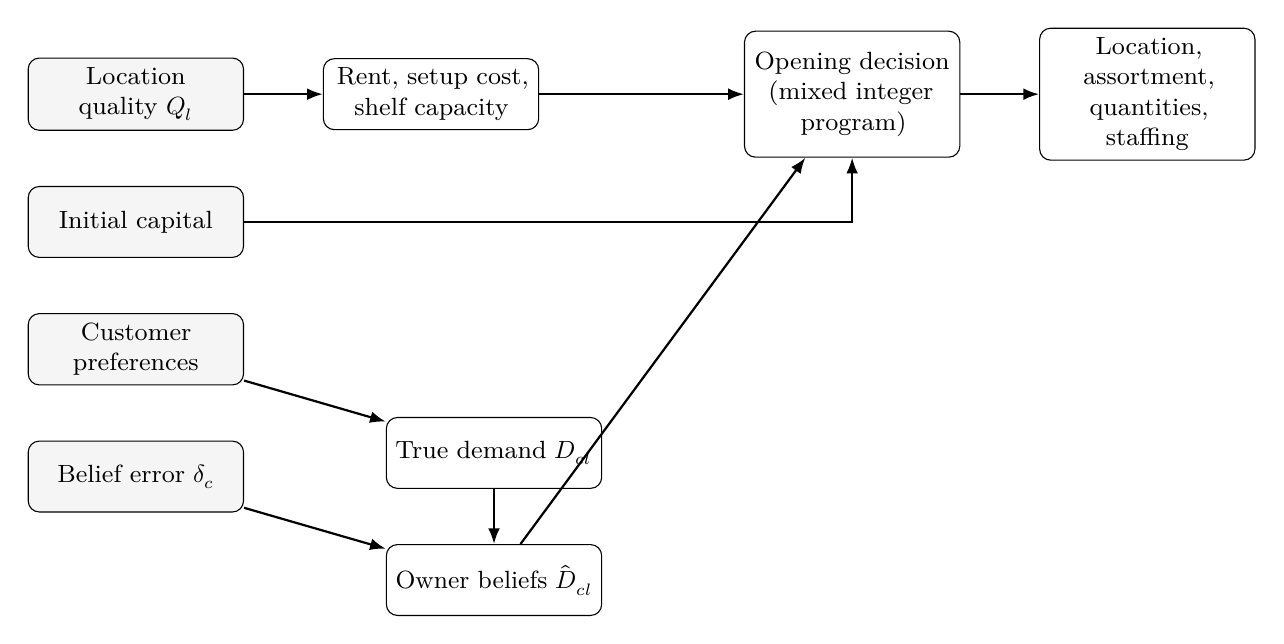
\begin{tikzpicture}[
    node distance = 7mm and 10mm,
    box/.style = {rectangle, draw, rounded corners, align=center, minimum height=0.9cm, font=\small, text width=2.5cm},
    exo/.style = {box, fill=black!4},
    arrow/.style = {-{Latex[length=2mm]}, thick}
]
    \node[exo] (Q) {Location quality $Q_l$};
    \node[exo, below=of Q] (K) {Initial capital};
    \node[exo, below=of K] (PREF) {Customer preferences};
    \node[exo, below=of PREF] (DELTA) {Belief error $\delta_c$};

    \node[box, right=of Q] (R) {Rent, setup cost, shelf capacity};
    \node[box, below right=4mm and 18mm of PREF] (D) {True demand $D_{cl}$};
    \node[box, below=of D] (BEL) {Owner beliefs $\hat{D}_{cl}$};

    \node[box, right=26mm of R, minimum height=1.6cm] (MILP) {Opening decision\\(mixed integer program)};

    \node[box, right=of MILP] (OUT) {Location, assortment,\\quantities, staffing};

    \draw[arrow] (Q) -- (R);
    \draw[arrow] (PREF) -- (D);
    \draw[arrow] (D) -- (BEL);
    \draw[arrow] (DELTA) -- (BEL);
    \draw[arrow] (R) -- (MILP);
    \draw[arrow] (BEL) -- (MILP);
    \draw[arrow] (K) -| (MILP);
    \draw[arrow] (MILP) -- (OUT);
\end{tikzpicture}
\caption{The causal skeleton of the opening decision. Everything upstream of the decision node is generative ground truth; the decision node and its consequences are the owner's boundedly rational response to it.}
\label{fig:phase1graph}
\end{figure}

Five specific divergences between belief and truth are built into this
one decision, and each is a documented, discoverable fact rather than an
arbitrary flaw: optimistic demand beliefs, a flat safety-stock rule
applied regardless of season, category-level markups that ignore
individual price sensitivity, static beliefs that never anticipate the
seasonal cycle of Section~\ref{sec:macro}, and a flat product-share cap
that ignores genuinely heterogeneous tastes. Section~\ref{sec:micro-adaptive}
shows what happens once Henrik starts learning from real sales instead
of belief alone, and Section~\ref{sec:counterfactual} shows exactly how
much that gap between belief and truth ends up costing him.

\subsection{The owner's day-to-day adaptive policies}
\label{sec:micro-adaptive}

Once the shop is open, Henrik stops guessing and starts watching. He
cannot see true demand any more now than he could on opening day --- he
only ever sees what actually sold, which is not the same thing, since a
stockout hides the sale that would have happened. What he does instead
is what any real shopkeeper does: he keeps an eye on what has been
selling lately, orders roughly that much again, marks down whatever is
piling up on the shelf, and worries about cash before he worries about
the annual accounts.

This is a genuinely different kind of decision from the opening
allocation, even though the same person makes both. It is repeated
weekly rather than made once, it responds to observed history rather than
to a belief formed in a vacuum, and it is deliberately a heuristic rather
than a re-optimization: Henrik does not re-solve a mixed integer program
every Monday morning, he applies a simple, realistic rule of thumb, the
same way a real shopkeeper does, and the rule's own blind spots are as
important to the model as its logic.

Once a week Henrik places a restocking order, sized off the simplest
forecast a real shopkeeper actually runs: a trailing four-week average
of his own recorded sales,

\[
\hat{D}^{\text{op}}_{cw} \overset{\leftarrow}{=} \frac{1}{4}\sum_{j=1}^{4}
\text{Sales}_{c,w-j} .
\]

He orders up to a target sized for the review and
lead time ahead of him, plus his standing safety-stock rule,
$\text{Target}_{sw} = \left(\tfrac{R+L}{7} + \eta\,\tfrac{30}{7}\right)
\hat{D}^{\text{op}}_{cw}\,\tilde{\sigma}_{sw}$, with $R=7$ days between
reviews, $L=2$ days of lead time, and $\tilde{\sigma}_{sw}$ the
product's smoothed recent share of its category. This rule carries two
realistic flaws built directly into its structure. It is backward
looking, so a rising seasonal trend is always underestimated by the
average of the weeks before it rose. And it is blind to censoring,
because the sales it averages are themselves truncated by the store's
own past stockouts, producing a self-reinforcing censoring spiral: a
product that stocks out repeatedly reports weak sales, earns a smaller
share of the next order, and stocks out again.

Henrik also runs two distinct kinds of promotion, and the contrast
between them is itself an intended lesson. A markdown campaign triggers
endogenously whenever a category's weeks of cover exceeds a threshold,
targeting the slowest-selling third of that category. Because the
trigger is overstock, and overstock correlates with weak underlying
demand, any naive before-and-after read of a markdown's effect is
contaminated by exactly the selection problem that afflicts real-world
marketing analytics. A separate, calendar-triggered storewide discount
on the last Sunday of every month is, by contrast, entirely exogenous ---
announced in advance and correlated with nothing about current stock ---
providing a clean source of price variation before anyone tries to
untangle the confounded markdowns.

Perishable stock spoils overnight,

\[
\text{Spoiled}_{st} \sim \text{Binomial}\big(\text{OnHand}_{st},\
\min(0.35,\ \lambda^d_{c(s)}\,f_{c(s),t})\big) ,
\]

with the spoilage factor $f_{ct}$
built from the same log-additive logic as every other multiplier in this
paper: a heat term strongest for ambient perishables such as bread and
produce, a cold-chain strain term loading on the macro shocks of
Section~\ref{sec:macro} and strongest for frozen and dairy goods, and an
idiosyncratic batch-luck term standing in for the reality that one
delivery simply travels worse than another. And Henrik's cash position
is tracked explicitly, with a credit line available whenever a month's
close would otherwise take cash below zero; restocking is itself capped
by available cash and credit headroom, so a struggling store visibly
thins its own shelves months before any trouble would show up in an
annual profit figure, exactly as a real distressed retailer's inventory
often signals difficulty well before its accounts do.

\subsection{The owner's expansion decision}
\label{sec:micro-expansion}

Sometime in Henrik's second year, if the business has been kind to him,
he faces a decision every real small-business owner eventually faces:
whether to risk some of what he has built on growing further. He does
not commission a discounted-cash-flow analysis of the decision. He
watches his own savings account. When it has grown past a point that
feels safe to risk, and only then, he hires his first employee, extends
his hours, and deepens his shelves.

This is neither the one-shot optimization of the opening decision nor
the weekly heuristic of ordinary restocking. It is a threshold decision
under genuine uncertainty about the future, and the threshold is framed
around what Henrik can actually afford to lose rather than around a
forecast of what the expansion will return --- much closer to what
entrepreneurship research calls \emph{effectuation}
(\hyperlink{ref:sarasvathy2001}{Sarasvathy, 2001}) than to a textbook net-present-value
calculation: a real small-business owner reasons from the resources
already in hand and the loss he can tolerate, not from a spreadsheet of
projected returns he has no reliable way to build.

From the beginning of the second year, Henrik retains a share $\rho_{RE}
= 0.5$ of every profitable month's after-tax result as declared retained
earnings, drawing the rest out as his own income,
$\text{draw}_m = (1-\rho_{RE})\,\max(0, \pi_m)$, and neither draws nor
retains anything in a loss month. Once retained earnings and available
cash both cross fixed thresholds, $\text{RE}_m \geq K_{\text{exp}}$ and
$\text{cash}_m - \text{tax\_reserve}_m \geq C_{\text{exp}}$, he expands
on the first day of the following month, paying a one-time fit-out cost
from savings.

The threshold $K_{\text{exp}}$ is calibrated so that, under the realized
path of the model, the expansion lands in the autumn of the second year
--- after a scripted local population increase but before a scripted
competitive entry the following year --- producing a specific and
analytically important narrative: the expansion looks entirely sensible
at the moment it is made, based on everything Henrik could reasonably
have known at the time, and only becomes questionable in hindsight once
a later, unrelated shock arrives. A counterfactual twin of the model, in
which the expansion threshold is disabled entirely, reveals that the
expansion's true cost across its first fourteen months substantially
exceeds the additional margin the extra hours and capacity actually
generate, because the fixed cost of an additional wage is paid in full
while the additional revenue it produces is diluted by the ordinary
grocery margin. This is a deliberately reproduced version of one of the
most common capital-allocation mistakes in small retail --- investing at
what retrospectively turns out to be the peak of the opportunity ---
generated here from the interaction of an ordinary retention rule, an
ordinary calibrated threshold, and an otherwise unrelated later shock,
rather than scripted as an explicit narrative choice.

\subsection{Population dynamics: the customer panel as a stochastic flow}
\label{sec:micro-panel}

Not every micro-level movement in this world is a decision in the sense
the last four sections meant. A neighborhood is not static: households
move in, households move out, and a shop's regulars are a population
in slow motion, not a fixed cast of characters. This is included in the
micro layer anyway, because it is exactly as emergent and exactly as
stochastic as everything above it, even though nobody is really
``choosing'' to leave the way Henrik chooses a price.

Structurally this is a renewal process: each customer has a type fixed
at creation that determines whether they are subject to departure risk
at all, departures happen at a constant hazard rate rather than on a
fixed schedule, and each departure is eventually replaced, so the
population's size is roughly stable even as its individual membership
turns over completely.

Each regular customer is given a persistence type drawn once,
rooted with probability $0.80$ and transient with probability $0.20$. A
rooted customer never leaves the neighborhood within the three-year
window at all; a transient customer faces an ongoing monthly hazard of
departure $h = 1/18$, a mean tenure of eighteen months. Every departure
is matched, after a delay of $1 + \text{Geometric}(0.5)$ months, by a
fresh household moving into the vacated home, and a slow trickle of
genuinely new arrivals, $\text{Poisson}(4)$ per year, represents modest
organic growth on top of straightforward replacement. Newly arrived
customers are drawn with an even fifty percent chance of either
persistence type, reflecting the reasonable assumption that a household
which has just moved once is more likely to move again than the settled
population it replaces.

Nothing about this churn is announced anywhere in the visible data; a
customer's card token simply stops appearing in the receipts one month
and never returns, and a new token begins appearing elsewhere. An
analyst must infer departure from silence, taking care not to confuse a
customer who has genuinely left with one merely visiting less often for
other reasons --- a distinction that becomes especially difficult near
the very end of the observed window, where a recently silent customer
cannot yet be told apart from one who will return next month. This is a
form of the right-censoring problem familiar from survival analysis, and
it is a genuine, unavoidable feature of any panel observed for a finite
length of time, reproduced here rather than glossed over.

\section{The Macro Layer: The Deterministic Script}
\label{sec:macro}

Everything in the previous section was computed fresh, each time the
world is run, from a decision-maker's own situation. Everything in this
section is the opposite: written down in advance, on a specific date,
completely independent of anything any customer or owner in the
simulation does. Weather does not care whether Henrik had a good month.
A competitor does not time its entry to Henrik's cash position. This
independence is not a simplifying convenience; it is what allows weather
to function as a natural experiment and a cost shock to function as an
instrument in later analysis, because nothing about the shop's own
behavior could possibly have caused the weather.

\subsection{Calendar and weather}

The simulated year runs three hundred sixty-five days, aligned to a real
calendar so seasons, holidays, and an analyst's ordinary intuitions all
line up, including two days on which the store is legally closed.
Temperature follows a deterministic annual cycle plus a persistent
stochastic anomaly, $T_t = \mu_T(t) + \varepsilon_t$ with $\mu_T(t) = 12
+ 9\cos\!\left(\tfrac{2\pi(t-200)}{365}\right)$ and $\varepsilon_t =
\phi\,\varepsilon_{t-1} + \text{Normal}(0,\sigma_\varepsilon)$,
$\phi=0.7$, an autoregressive form chosen because it is the maximum
entropy stationary process consistent with exactly the two facts about
weather worth encoding: a stable typical spread, and warm or cold spells
that persist for several days rather than resetting each morning. The
decomposition into a deterministic cycle and a stochastic anomaly is
itself a causal design choice: it lets a later analysis distinguish the
predictable effect of season from the genuinely surprising effect of
weather, since the anomaly is built orthogonal to the calendar, while in
raw data the two are thoroughly entangled, because July is warm
precisely because it is July.

Rainfall needs two separate decisions, whether it rains at all and how
much, each with its own natural distribution. Occurrence follows a
two-state Markov chain, $W_t \mid W_{t-1} \sim \text{Bernoulli}\big(
p_{01}(1-W_{t-1}) + p_{11}\,W_{t-1}\big)$ with $p_{01}=0.25$,
$p_{11}=0.55$, because weather fronts pass through and wet days genuinely
cluster, which an independent coin flip at every day cannot represent;
these transitions imply a stationary wet-day frequency of about
thirty-six percent and wet spells averaging just over two days, both
ordinary for a temperate climate. Given rain, the amount follows
$R_t \mid W_t{=}1 \sim \text{Gamma}(1.4, \text{mean}=5\text{ mm})$, the
standard meteorological choice, producing the realistic pattern of many
light drizzles and few genuine downpours.

\subsection{Category demand and foot traffic}

A daily, per-category demand modifier $M_{ct}$ scales how strongly the
neighborhood wants a given category on a given day, built log-additively
from three genuinely distinct causal channels, $\log M_{ct} = a_c
\cos\!\left(\tfrac{2\pi(t-200)}{365}\right) + \kappa_c\, z_t + h_c\, H_t$,
where $z_t$ is the standardized temperature anomaly and $H_t$ flags days
before a major holiday. The seasonal amplitude $a_c$ captures the
predictable annual cycle; the anomaly loading $\kappa_c$ captures the
pure weather effect, an unseasonably warm week moving demand right now
regardless of the calendar; the holiday loading $h_c$ captures the
stock-up surge before a major holiday. One category is deliberately
given all-zero loadings, so nothing in preferences makes it more or less
wanted at any time of year; its observed sales are nevertheless not
perfectly flat, because every category draws from the same household
budget, and when other categories surge seasonally they crowd the flat
category out. An analyst who finds an apparent seasonal pattern here and
stops has mistaken a budget-mediation effect for a genuine preference
effect. A small number of specific product types whose seasonality
flagrantly contradicts their category's average, such as ice cream,
receive their own finer-grained tilt, $\log \psi_{pt} = a_p
\cos\!\left(\tfrac{2\pi(t-200)}{365}\right) + \kappa_p\, z_t$, entering
the discrete-choice utility of Section~\ref{sec:micro-customer} directly
as $U_{ist} = U_{is} + \log\tilde{\psi}_{p(s),t}$.

Weather does not only change what people buy; it changes whether they
come at all. A daily traffic modifier, $\log \Lambda_t = -0.20\,W_t +
0.15\,H_t + \varepsilon^{\Lambda}_t$ with the same autoregressive
persistence as temperature ($\phi^\Lambda = 0.85$), scales every
customer's visit probability down by about eighteen percent on a wet
day and up by about sixteen percent before a major holiday. A subtle
consequence follows automatically from the pantry mechanism of
Section~\ref{sec:micro-customer}: because a customer's need for a
category grows with time since their last purchase, a customer rained
off on one day simply arrives hungrier a few days later. The familiar
retail pattern of a dip on the rainy day followed by a rebound emerges
purely from two mechanisms that never reference each other, with no
separate rebound parameter anywhere in the model.

Household budgets move too. Each week's budget is $B_{iw} = B_i \cdot
e^{\xi_{iw}} \cdot s_{iw} \cdot g_{iw}$, with an ordinary weekly wobble
$\xi_{iw} \sim \text{Normal}(0, 0.12)$ and two rarer, more consequential
terms: a tight spell sets $s_{iw}=0.65$ for a genuine hardship such as a
job loss, beginning with probability $0.004(1+2\bar{g}_w)$ per week and
persisting a memoryless $\text{Geometric}(1/6)$ further weeks, where
$\bar{g}_w$ is the scripted energy crisis's own trajectory below; a
splurge sets $g_{iw}=1.5$ for a single week with probability $0.01$. The
tight spell's entry rate is deliberately coupled to the crisis
trajectory, tripling at its peak, because a real energy crisis squeezes
household heating bills at the same time as it squeezes a retailer's
refrigeration costs.

\subsection{Macroeconomic cost shocks}

Beneath the everyday weather sits a slower-moving layer of wholesale
cost shocks, and beneath that a continuous inflation drift,
$\text{infl}(t) = e^{\pi t /365}$ with $\pi=0.025$ a year. Shocks proper
arrive as a marked point process: $K \sim \text{Poisson}(1.5)$ events,
each at $\tau_k \sim \text{Uniform}(1,365)$, a Poisson count because it
is the maximum entropy distribution for a number of rare independent
events given only a rate, with a well-known property of the Poisson
process guaranteeing that, given the count, arrival times are
conditionally uniform across the year --- a theorem, not an additional
assumption. One large event, an autumn energy crisis, is scripted rather
than drawn at random, so every run tells a genuinely interesting
supply-side story. Each event's peak magnitude is $\zeta_k \sim
\text{LogNormal}(\log\zeta_0,\ 0.3)$, and its effect over time is
$g_k(t) = \zeta_k \cdot \min(1, (t-\tau_k)/14) \cdot \exp(-(t-\tau_k-14)_+/\rho_k)$,
ramping up over two weeks and decaying exponentially, neither a
permanent level change nor a transient blip but a slow wave a forecaster
genuinely has to track. Every affected category's cost multiplier then
assembles the drift and every live shock, $\log \text{CostMult}_{ct} =
\pi t/365 + \sum_k g_k(t)\,\mathbb{1}[c \in A_k]$.

Henrik never observes $\text{CostMult}_{ct}$ directly; he sees only his
supplier's invoices, and tracks an exponentially smoothed trend,
$\overline{\text{Cost}}_{s,t} = \alpha\,\text{Cost}_{s,t} +
(1-\alpha)\,\overline{\text{Cost}}_{s,t^-}$, $\alpha=0.35$, moving the
shelf tag only once the smoothed cost has drifted more than three
percent from the current price --- menu-cost pricing, a pattern well
documented in the economics literature. The consequence is that shelf
prices vary over time for reasons entirely unconnected to the demand
side of the market: a foreign harvest failure moves costs without
touching any household's budget, exactly the exogenous price variation
an econometrician needs to estimate a genuine price elasticity rather
than a number contaminated by reverse causation. The scripted energy
crisis is a deliberate exception to this cleanliness, since it also
squeezes household budgets through the tight-spell mechanism above,
making it a subtly invalid instrument whose bias can, in principle, be
computed exactly.

\begin{figure}[htbp]
\centering
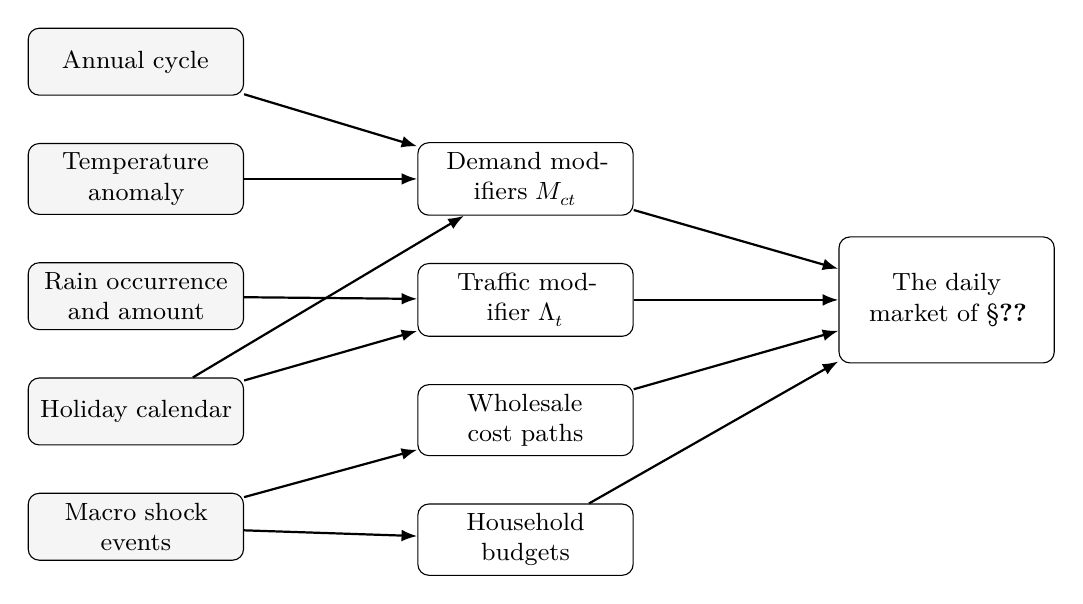
\begin{tikzpicture}[
    node distance = 6mm and 8mm,
    box/.style = {rectangle, draw, rounded corners, align=center, minimum height=0.85cm, font=\small, text width=2.5cm},
    exo/.style = {box, fill=black!4},
    arrow/.style = {-{Latex[length=2mm]}, thick}
]
    \node[exo] (SEA) {Annual cycle};
    \node[exo, below=of SEA] (ANOM) {Temperature anomaly};
    \node[exo, below=of ANOM] (RAIN) {Rain occurrence and amount};
    \node[exo, below=of RAIN] (HOL) {Holiday calendar};
    \node[exo, below=of HOL] (EVT) {Macro shock events};

    \node[box, right=22mm of ANOM] (M) {Demand modifiers $M_{ct}$};
    \node[box, below=of M] (LAM) {Traffic modifier $\Lambda_t$};
    \node[box, below=of LAM] (CM) {Wholesale cost paths};
    \node[box, below=of CM] (BW) {Household budgets};

    \node[box, right=26mm of LAM, minimum height=1.6cm] (P3) {The daily\\market of \S\ref{sec:micro-customer}};

    \draw[arrow] (SEA) -- (M);
    \draw[arrow] (ANOM) -- (M);
    \draw[arrow] (HOL) -- (M);
    \draw[arrow] (RAIN) -- (LAM);
    \draw[arrow] (HOL) -- (LAM);
    \draw[arrow] (EVT) -- (CM);
    \draw[arrow] (EVT) -- (BW);

    \draw[arrow] (M) -- (P3);
    \draw[arrow] (LAM) -- (P3);
    \draw[arrow] (CM) -- (P3);
    \draw[arrow] (BW) -- (P3);
\end{tikzpicture}
\caption{The causal skeleton of the macro layer. Every arrow points into the daily market that Section~\ref{sec:micro-customer} performs; nothing points back, which is what licenses treating these channels as exogenous instruments and natural experiments.}
\label{fig:phase2graph}
\end{figure}

\subsection{Taxation as scripted policy}
\label{sec:macro-tax}

A policy laboratory without taxation would be unable to represent the
most common lever through which real macroeconomic policy actually
reaches individual households and businesses, so a complete, differentiated
tax system sits in the baseline world itself, exactly as scripted and
exactly as exogenous as the weather above. Value-added tax applies at a
category-specific rate $r_c(t)$, and Henrik's shelf tag is formed from
the tax-exclusive, smoothed invoice cost with the current rate reapplied
on top, $\text{Tag}_{st} = \text{charm}\big(\overline{\text{NetCost}}_{s,t}
\cdot (1+m_c)(1+r_c(t))\big)$. Because the rate enters multiplicatively
on the trend he already tracks, a rate change reaches his \emph{intended}
price immediately and exactly, while the price customers actually see
continues to lag through the same menu-cost mechanism above --- exactly
the kind of incomplete, delayed tax pass-through documented in the
empirical public finance literature. Value-added tax is remitted monthly
as the difference between output tax on sales and input tax on
purchases, $\text{VAT}_t = \sum_c \text{Sales}_{ct}\,r_c/(1+r_c) -
\sum_c \text{Purchases}_{ct}\,r_c/(1+r_c)$; payroll tax applies to wages
at a flat employer rate $r^{\text{pay}}=0.25$; and a flat tax applies to
positive annual profit only, accrued in the year it is earned,
$\text{ProfitTax} = r^{\pi}\cdot\max(0,\text{ProfitBeforeTax})$,
$r^\pi=0.20$.

Henrik is tax-aware but not tax-strategic: he correctly prices on his
net-of-tax margin and correctly accounts for the full employer cost of
hiring in his opening decision, but he never performs cross-category tax
arbitrage or elasticity-aware repricing in response to a tax change,
leaving that gap as an open door for a later prescriptive analysis to
identify and price. One piece of this is provably harmless rather than
merely assumed away: because profit tax is a flat rate on a positive
base, $\arg\max_{\text{decisions}} (1-r^\pi)\pi(\text{decisions}) =
\arg\max_{\text{decisions}} \pi(\text{decisions})$, so an owner who
ignores profit tax when making ordinary operating decisions loses
nothing relative to one who optimizes around it. No such guarantee holds
for value-added tax, whose category-specific rate changes relative
prices across categories and can, in principle, reward cross-category
arbitrage Henrik never performs.

\subsection{A world that stays unquiet}

A scenario, in this model, is nothing more than a declarative edit to
one of the quantities this section already defined: an extra cost event
riding the same trajectory $g_k(t)$ above, a multiplier on the traffic
modifier $\Lambda_t$, a multiplier on household budgets $B_{iw}$, or a
new tax rate path $r_c(t)$ from a given date. A scenario never edits an
underlying random-number stream directly, only the script. Consistent
with the design principle that a three-year history should not read as
a single stable year merely repeated three times, the second and third
years of Henrik's story are populated with a specific sequence of such
edits, each chosen to test a distinct analytical skill: an equipment
failure destroying frozen and refrigerated stock overnight, a
single-category cost shock on dairy, a prolonged summer heatwave, a
scripted local population increase, a contractual rent increase at a
two-year lease renewal alongside similarly lumpy, dated steps in wages
and utilities, and the entry of a discounting competitor a short
distance away.

That competitor's effect on individual customers is deliberately
heterogeneous,

\[
m_i = \exp(-\chi\cdot\tilde{s}_i\cdot k_i) ,
\]

a multiplicative penalty on visit probability where $\tilde{s}_i$ is a
customer's percentile rank in price sensitivity and $k_i = 1.0$ for
transient customers but only $0.6$ for rooted ones, so the competitor
draws away price-sensitive customers fastest, and customers held by
relationships rather than price alone are penalized at only sixty
percent of the rate a transient customer at the same price sensitivity
would be. It is followed by a scheduled, rather than reactive, pricing
response, a short seasonal street festival, and a second cost shock on
staple goods.

\section{Why the Split Licenses Counterfactual Reasoning}
\label{sec:counterfactual}

Every decision in Section~\ref{sec:micro} and every script in
Section~\ref{sec:macro} was built the way it was for one reason that
this section finally makes explicit. Because the macro layer is written
entirely in advance and never listens to anything the micro layer does,
a counterfactual world can be produced almost for free: edit the script
--- delete the scripted energy crisis, disable the expansion threshold,
remove the competitor entirely --- and replay the identical daily market
mechanism with every other random draw held fixed. The difference
between the original run and the edited run is then the causal effect
of the edit itself, not merely an estimate of it.

This only works because of a discipline that has been present, silently,
in every equation in this paper: every random draw is keyed by the
stable identity of the entity it concerns, a specific customer on a
specific day, a specific product on a specific night, using
independently spawned child streams, rather than one long sequential
stream. If every draw were taken sequentially, deleting a single event
partway through the year would shift every subsequent draw, and the
comparison between two runs would be contaminated by reshuffled
randomness that has nothing to do with the edit itself. Keying every
draw by identity means a customer untouched by the edit reproduces the
identical decision, bit for bit, in both runs --- the common random
numbers technique familiar from the simulation literature, adopted from
the first line of the implementation rather than retrofitted later,
because retrofitting it afterward would require rewriting every random
draw in the model.

Two concrete pairs of counterfactual twins in Henrik's own three-year
story cash this discipline out into an actual number rather than a
methodological promise. One twin disables the expansion threshold of
Section~\ref{sec:micro-expansion} entirely; comparing it to the real
run reveals that the expansion's true cost across its first fourteen
months substantially exceeds the additional margin it generates. A
second twin removes the competitor of Section~\ref{sec:macro} entirely;
comparing it to the real run prices exactly what the competitor cost
Henrik, as opposed to what he believes it cost him. A specific, intended
finding of the model is that the capital decision very often costs the
business substantially more than the competitive entry does, even
though the competitor is the more visible and more emotionally salient
event to an owner living through it --- which is exactly why an
instructor can hand a learner Henrik's own conviction that the
competitor is to blame, and let the two counterfactual twins settle the
question the data, rather than the instructor, gets to answer.

With a full year performed, three profit figures become computable side
by side: what Henrik believed he would earn at the moment of opening,
$\pi_{\text{believed}}$, read directly off the opening decision's own
objective value; what the ledger actually shows after a full year of
realistic behavior, $\pi_{\text{realized}}$, the number a real
accountant would certify; and what a perfectly informed operator could
have earned given the same world --- the same customers, the same
script, the same policy shapes, but true demand in place of Henrik's
censored, backward-looking forecast --- $\pi_{\text{oracle}}$. The two
gaps between these figures are exact differences between fully computed
runs of the same mechanism, $\Delta_{\text{optimism}} =
\pi_{\text{realized}} - \pi_{\text{believed}}$ and
$\Delta_{\text{analytics}} = \pi_{\text{oracle}} - \pi_{\text{realized}}$,
where the first measures the cost of Henrik's initial overoptimism and
the second measures the value of better information and better
decisions --- the single number this entire construction exists to make
credible by actually computing it, rather than merely asserting a
plausible size for it.

\section{Recording and Accounting: An Imperfect Window on a Perfect World}
\label{sec:recording}

Everything described so far --- every decision, every script --- happens
inside a simulated reality that is always exactly conserved: every unit
that is bought is eventually sold, spoiled, or counted, and every euro
that moves is accounted for somewhere. An early, fully reconciled version
of this dataset was reviewed and found, on inspection, to have one
serious flaw: its records were perfect. Revenue tied to the cent, every
inventory identity closed exactly, and no document was ever missing,
duplicated, or mistyped. Real bookkeeping is never like this, and a
dataset that reconciled perfectly would itself be evidence of
fabrication to any experienced reader.

The paperwork therefore sits in a third layer of this model, neither a
decision nor a script: a small number of realistic paperwork defects,
injected at low, carefully calibrated rates only at the point of export,
never touching the simulation's own internal state. A point-of-sale
terminal retries an upload and duplicates a till receipt. A distracted
clerk posts the same invoice twice. A delivery is paid for but never
logged. Unrecorded spoilage surfaces only later as unexplained monthly
shrinkage. An inventory count is mistyped and self-corrects the
following night. Each defect is drawn from its own independently keyed
stream and simultaneously written to a separate answer key recording
exactly what was changed, so the exercise of reconciling the messy
records back to the truth is itself gradable against a known answer,
and the underlying simulated reality that Section~\ref{sec:counterfactual}'s
counterfactual machinery depends on is never disturbed by paperwork
noise that exists only in the documents an analyst receives.

This drift has its own exact algebra. Let $D_{st}$ denote a product's
cumulative book-minus-true discrepancy on day $t$, pushed upward by
duplicate invoices and unrecorded spoilage and downward by missing
invoices and duplicate receipts. The inventory figure an analyst actually
sees is book stock rather than true stock,
$B_{st} = S_{st} + D_{st} - \sum_{c\le t} A_{sc}$, where $A_{sc}$ is the
cumulative correction posted at each monthly physical count, which snaps
the book back to physical truth before it begins drifting anew. Genuine
refunds are kept deliberately separate from this recording layer and
modeled instead as a true simulation event: after each receipt is
finalized, an independently keyed stream decides whether one of its
lines is returned, $\Pr(\text{refund}\mid\text{receipt}) = 0.006$, with
the return posted days later as its own till transaction, referencing
the original receipt, destroying rather than restocking the returned
unit.

The same discipline governs money. Revenue is recognized on a cash basis
at the moment of sale, at the price actually paid after any live
markdown. A voided mis-ring, in which a cashier corrects an immediate
scanning error, nets to zero money and zero goods and is distinguishable
from a genuine refund by the absence of a reference to an earlier
receipt. Book stock is governed by a strict identity, $\text{book}(t) -
\text{book}(t-1) = \text{deliveries}(t) - \text{sales}(t) -
\text{write\_offs}(t)$, with any deviation traceable either to a
deliberate recording defect or to the monthly physical count. Perishable
spoilage and monthly count corrections are kept in strictly separate
categories because they measure two different things, genuine physical
waste and pure bookkeeping drift, and conflating them would double-count
the same euros. The monthly ledger aggregates revenue, procurement,
rent, wages, utilities, storage, promotional costs, net tax, and credit
interest into a single bottom line, made explicit at the annual horizon
as

\begin{align*}
\text{ProfitBeforeTax} \overset{\leftarrow}{=}\ & \sum \text{Revenue} -
\sum\big(\text{Procurement} + \text{Rent} + \text{Wages}\big) \\
&\quad {} - \sum\big(\text{PayrollTax} + \text{Utilities} +
\text{Storage}\big) \\
&\quad {} - \sum\big(\text{Flyers} + \text{VAT} +
\text{CreditInterest}\big) - \text{Openings},
\end{align*}

with profit tax levied only on a genuine surplus,
$\text{ProfitTax} = 0.20\times\max(0,\text{ProfitBeforeTax})$ and
$\text{ProfitAfterTax} = \text{ProfitBeforeTax} - \text{ProfitTax}$, so a
loss year triggers no tax liability but also earns no rebate, mirroring
the asymmetric treatment a real small proprietorship faces. The rule
that makes every part of this paper trustworthy at once is this: the
owner's own monthly ledger is always correct about money, and every
other document --- particularly the raw till receipts and the raw
supplier invoices --- is the analyst's own paperwork to reconcile
against it.

\section{Design Principles and Notation}
\label{sec:principles}

A few conventions recur so often in the sections above that it is worth
naming them once, plainly, rather than re-explaining them at every
occurrence.

\subsection{The three-question discipline}

Every stochastic element in this paper, from a customer's weekly grocery
budget to the day a storm arrives, was chosen by answering the same
three questions, in the same order. What values can the variable
actually take --- its \emph{support}? A probability must live on
$(0,1)$; a count must be a nonnegative integer; a cost must be strictly
positive. What \emph{generative story} actually produces it? A quantity
built from many small effects adding together behaves differently from
one built from many small factors multiplying together, and both differ
from one built from a fixed number of independent yes-or-no trials.
And, once support and story have narrowed the field, which distribution
within it is \emph{maximum entropy} --- adds the least unwarranted
structure beyond the facts actually being claimed? This discipline
explains a pattern that recurs throughout this paper: a budget built
from many small multiplicative factors is LogNormal; a probability such
as a schedule-adherence rate is Beta; a count of rare independent events
such as a shock arrival is Poisson. None of these choices are arbitrary
or repeated by habit; each answers the same three questions afresh in
its own context.

\subsection{Notation}

Distributions are written with their natural parameters throughout, so a
Normal distribution is always $\text{Normal}(\mu,\sigma)$ and never
$\text{Normal}(\mu,\sigma^2)$. The symbol $\sim$ denotes a stochastic
draw; $=$ denotes a deterministic definition; and
$\overset{\leftarrow}{=}$ is reserved for the cost and accounting
identities, where the direction of causation is itself the point being
made. A hat, $\hat{\cdot}$, always marks a belief held by the owner, as
opposed to the corresponding true value he cannot observe. Locations are
indexed by $l$, categories by $c$ (twelve, matching a real product
catalog), products by $s$, customers by $i$, and days by $t$; weeks by
$w$, months by $m$, and shock events by $k$. A small number of letters
are reused across sections for unrelated quantities exactly as they are
reused in the underlying implementation --- $\alpha$, $m$, and $\chi$
each mean something different depending on where they appear --- and
every such reuse is flagged in prose at the point it recurs.

\subsection{Reproducibility}

The entire model is driven by a single seeded pseudorandom generator, so
the whole three-year history is reproducible exactly from one integer,
and the keyed-randomness discipline of Section~\ref{sec:counterfactual}
is what turns that reproducibility into genuine counterfactual power
rather than mere determinism.

\section{Discussion}
\label{sec:discussion}

Four choices recur across every section of this paper and are worth
drawing out explicitly, because they explain why the architecture as a
whole looks the way it does rather than some equally plausible
alternative.

The first is that every random variable is defended on its own terms by
the three-question discipline, rather than by convention or
convenience, which means the size and shape of every planted pattern in
the data --- the degree of overstocking caused by Henrik's optimism, the
seasonal swing in a particular product's sales --- can in principle be
computed exactly from the model's own parameters rather than merely
observed empirically after the fact.

The second is the strict separation between the micro layer of
Section~\ref{sec:micro} and the macro layer of Section~\ref{sec:macro}:
what is decided fresh each time the world runs, and what is written down
in advance and never listens to anything the simulated people do. This
is what allows weather and macroeconomic shocks to function as
instruments and natural experiments, and it is what allows an owner's
documented mistakes to be genuine, traceable consequences of otherwise
reasonable behavior rather than arbitrary flaws inserted for pedagogical
convenience.

The third is the strict separation, laid out in
Section~\ref{sec:recording}, between the underlying physical reality of
the simulated world, always internally consistent and exactly conserved,
and the paperwork describing that reality, which is allowed to be
imperfect in the same limited, realistic ways real business paperwork
is imperfect. This is what allows the counterfactual machinery of
Section~\ref{sec:counterfactual} to remain exact even in the presence of
realistic recording noise, because that noise is injected only at the
point of export and never touches the simulated state itself.

The fourth is that a small number of specific, deliberate gaps between
belief and truth --- an owner's demand estimate, his forecasting rule,
his tax strategy, his capital-allocation decision --- are each
introduced once, defended on realistic grounds, and then left
undisturbed rather than corrected. This is a deliberate design stance
rather than an oversight: the entire point of this construction is to
produce a world in which the distance between what an agent believes
and what is true can be measured precisely, and that distance can only
be measured if the model resists the temptation to make its own
protagonist smarter than the premise requires.

\section{Conclusion}
\label{sec:conclusion}

This paper has told the story of a simulated grocery store as a
collection of decisions rather than a chronology of software phases:
what a customer wants at a shelf, what an owner believes before a
single sale exists, how that owner adjusts once real sales do exist,
when he dares to risk capital on growing further, and how a whole
neighborhood drifts in and out of being his customers, set against a
macro layer that is scripted, deterministic, and never listens to any
of it. Every one of those decisions was built the same way: from the
plain intuition a real person would give you if you asked them why, to
the precise mathematical object that intuition becomes. The result is a
world in which an observable pattern --- a seasonal swing in ice cream
sales, an overstocked category, a capital decision that looks reasonable
at the time and questionable in hindsight --- always traces back to one
of these decisions or scripts rather than to an arbitrary injection of
noise, and in which the gap between what somebody believed and what
was actually true can, for the first time, be measured rather than
merely argued about. Readers who want the precise specification behind
any single mechanism sketched here, at a level suitable for
reimplementation, should turn to \texttt{documents/PHASE1\_DETAILS.md}
through \texttt{PHASE5\_DETAILS.md} in the project repository; this
paper's job was only ever to explain why each of those mechanisms is
there, and what it is like to live inside the economy they add up to.

\section*{References}
\addcontentsline{toc}{section}{References}

\begin{list}{}{\leftmargin=1.5em \itemindent=-1.5em \itemsep=8pt}

\item \hypertarget{ref:dwork2006}{}Dwork, C. (2006). Differential privacy.
In \textit{Proceedings of the 33rd International Colloquium on Automata,
Languages and Programming (ICALP)}, Part II, Lecture Notes in Computer
Science vol.\ 4052, 1--12. Springer.

\item \hypertarget{ref:mcfadden1974}{}McFadden, D. (1974). Conditional
logit analysis of qualitative choice behavior. In P. Zarembka (Ed.),
\textit{Frontiers in Econometrics}, 105--142. Academic Press.

\item \hypertarget{ref:orcutt1957}{}Orcutt, G. H. (1957). A new type of
socio-economic system. \textit{Review of Economics and Statistics}, 39(2),
116--123.

\item \hypertarget{ref:patki2016}{}Patki, N., Wedge, R., and
Veeramachaneni, K. (2016). The synthetic data vault. In \textit{Proceedings
of the IEEE International Conference on Data Science and Advanced Analytics
(DSAA)}, 399--410.

\item \hypertarget{ref:sarasvathy2001}{}Sarasvathy, S. D. (2001).
Causation and effectuation: Toward a theoretical shift from economic
inevitability to entrepreneurial contingency. \textit{Academy of
Management Review}, 26(2), 243--263.

\item \hypertarget{ref:xu2019}{}Xu, L., Skoularidou, M., Cuesta-Infante,
A., and Veeramachaneni, K. (2019). Modeling tabular data using conditional
GAN. In \textit{Advances in Neural Information Processing Systems 32
(NeurIPS 2019)}, 7335--7345.

\end{list}

\end{document}
